\documentclass[12pt]{article}
\usepackage[margin=1in]{geometry}
\usepackage{graphicx}
\usepackage{hyperref}
\usepackage{booktabs}
\usepackage{amsmath}
\usepackage{caption}
\usepackage{float}
\usepackage[backend=biber,style=ieee]{biblatex}
\addbibresource{references.bib}

\title{A Stochastic Motorsport Performance Simulator:\\Final Report (Milestone 5)}
\author{Bryan Juarez Hernandez\\CS 4632 Modeling and Simulation\\Kennesaw State University}
\date{April 30, 2026}

\begin{document}
\maketitle
\begin{center}
GitHub Repository: \url{https://github.com/bryanhdzksu/CS4632_RACING_SIM.git}
\end{center}

\begin{abstract}
This project presents a stochastic motorsport performance simulator that analyzes race outcomes under uncertainty by combining physics-inspired deterministic modeling with Monte Carlo experimentation. The simulator captures aerodynamic drag/downforce tradeoffs, friction-limited cornering, tire-weather interaction, visibility penalties, and driver variability, then aggregates results across repeated trials to estimate lap-time distributions, expected race performance, and win probabilities rather than single deterministic outcomes.

The final system is modular and reproducible: simulation scenarios are defined through JSON configurations, executed through a reusable core engine, and exported as structured CSV/JSON artifacts including configuration snapshots, summary statistics, lap-level time series, and segment-level event logs. The implementation also generalizes to an arbitrary number of entrants, enabling broader scenario design and more flexible comparative analysis across race conditions.

Sensitivity studies were performed across five parameters (wetness, visibility, number of laps, trial count, and track complexity). Results show wetness is the dominant environmental driver of race-time change, while visibility has smaller but measurable effects. Trial-count experiments further demonstrate that increasing Monte Carlo samples improves confidence interval stability and strengthens reliability of conclusions. Overall, the project delivers a complete end-to-end simulation and analysis pipeline suitable for educational modeling and simulation, while providing clear extension paths for future work such as tire degradation, pit-stop strategy, richer powertrain dynamics, and deeper empirical calibration.
\end{abstract}

\newpage
\tableofcontents
\listoffigures
\listoftables
\newpage

\section{Introduction}
Motorsport outcomes emerge from tightly coupled nonlinear effects among vehicle setup, track geometry, environment, and human performance. Small changes in friction or visibility can shift cornering constraints, braking behavior, and strategic competitiveness over race distance. The core challenge is that deterministic single-run outputs are not enough: stakeholders need distributions of outcomes under uncertainty.

This project asks three research questions:
\begin{enumerate}
    \item How sensitive are race-time and win-probability outputs to key environmental and simulation parameters?
    \item Can a computationally lightweight physics-inspired model still produce defensible and interpretable trends?
    \item How does stochastic driver variability alter expected outcomes compared with purely deterministic modeling?
\end{enumerate}

The project objective is to build a reproducible simulation framework that provides insight into setup-performance tradeoffs, not to recreate full real-time vehicle dynamics or esports-grade control fidelity.

\section{Background and Literature Review}
The theoretical basis follows established modeling themes: aerodynamic force relationships, friction-limited motion, segment-based lap-time decomposition, and stochastic outcome analysis.

Vehicle dynamics references informed the drag/downforce and cornering limits \cite{ucsd_vehicle_dynamics}. Tire-road behavior was informed by Pacejka concepts, though implemented here with simplified friction coefficients for tractability \cite{pacejka}. Aerodynamic tradeoffs were motivated by road-vehicle drag/downforce notes \cite{mcgann_drag}. Segment accumulation logic follows race lap-time simulation framing from Bonfim \cite{bonfim_thesis}. Stochastic race modeling and Monte Carlo convergence concepts draw on motorsport-focused and general Monte Carlo references \cite{sulsters_f1,kroese_mc}. Driver variability framing aligns with lightweight agent-based modeling ideas \cite{wilensky_abm}.

The implemented model intentionally simplifies full nonlinear tire curve and drivetrain systems to match course scope while preserving interpretable cause-effect relationships.

\section{Model Design and Architecture}
The final architecture contains separate modules for configuration, domain entities, simulation execution, and data export.

\subsection{Conceptual Model}
Each race consists of:
\begin{itemize}
    \item Track segments (alternating straights/corners),
    \item Environment state (weather, wetness, visibility),
    \item Entrants (driver + car + tire),
    \item Repeated Monte Carlo trials for probabilistic outcomes.
\end{itemize}

\subsection{Updated UML}
\begin{figure}[H]
    \centering
    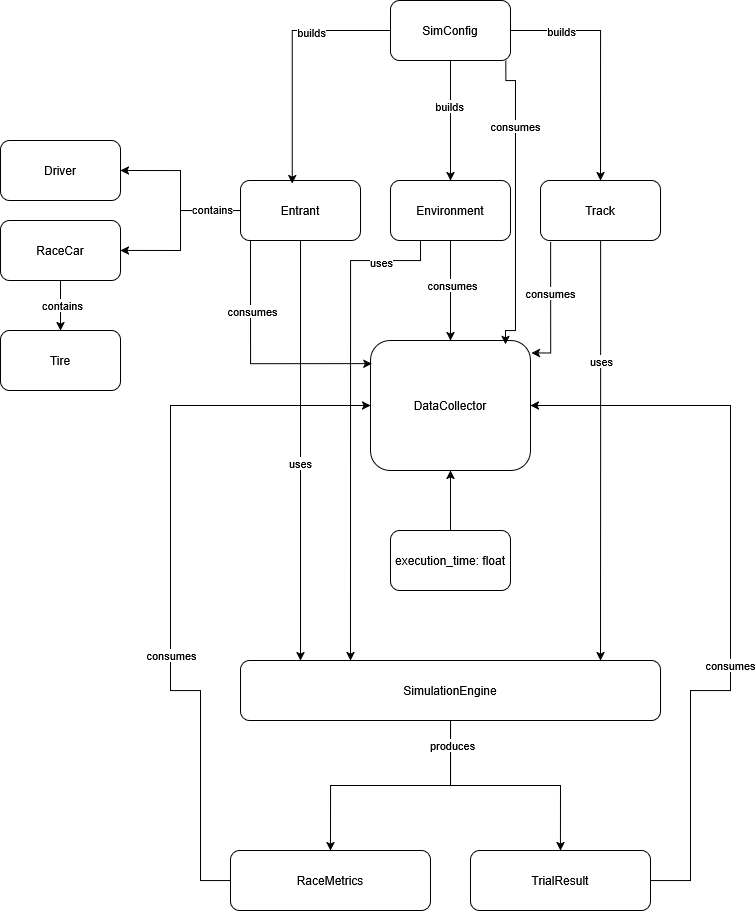
\includegraphics[width=\textwidth]{figures/updated_uml_class_diagram.png}
    \caption{Updated UML class diagram for the final implementation.}
\end{figure}

\begin{figure}[H]
    \centering
    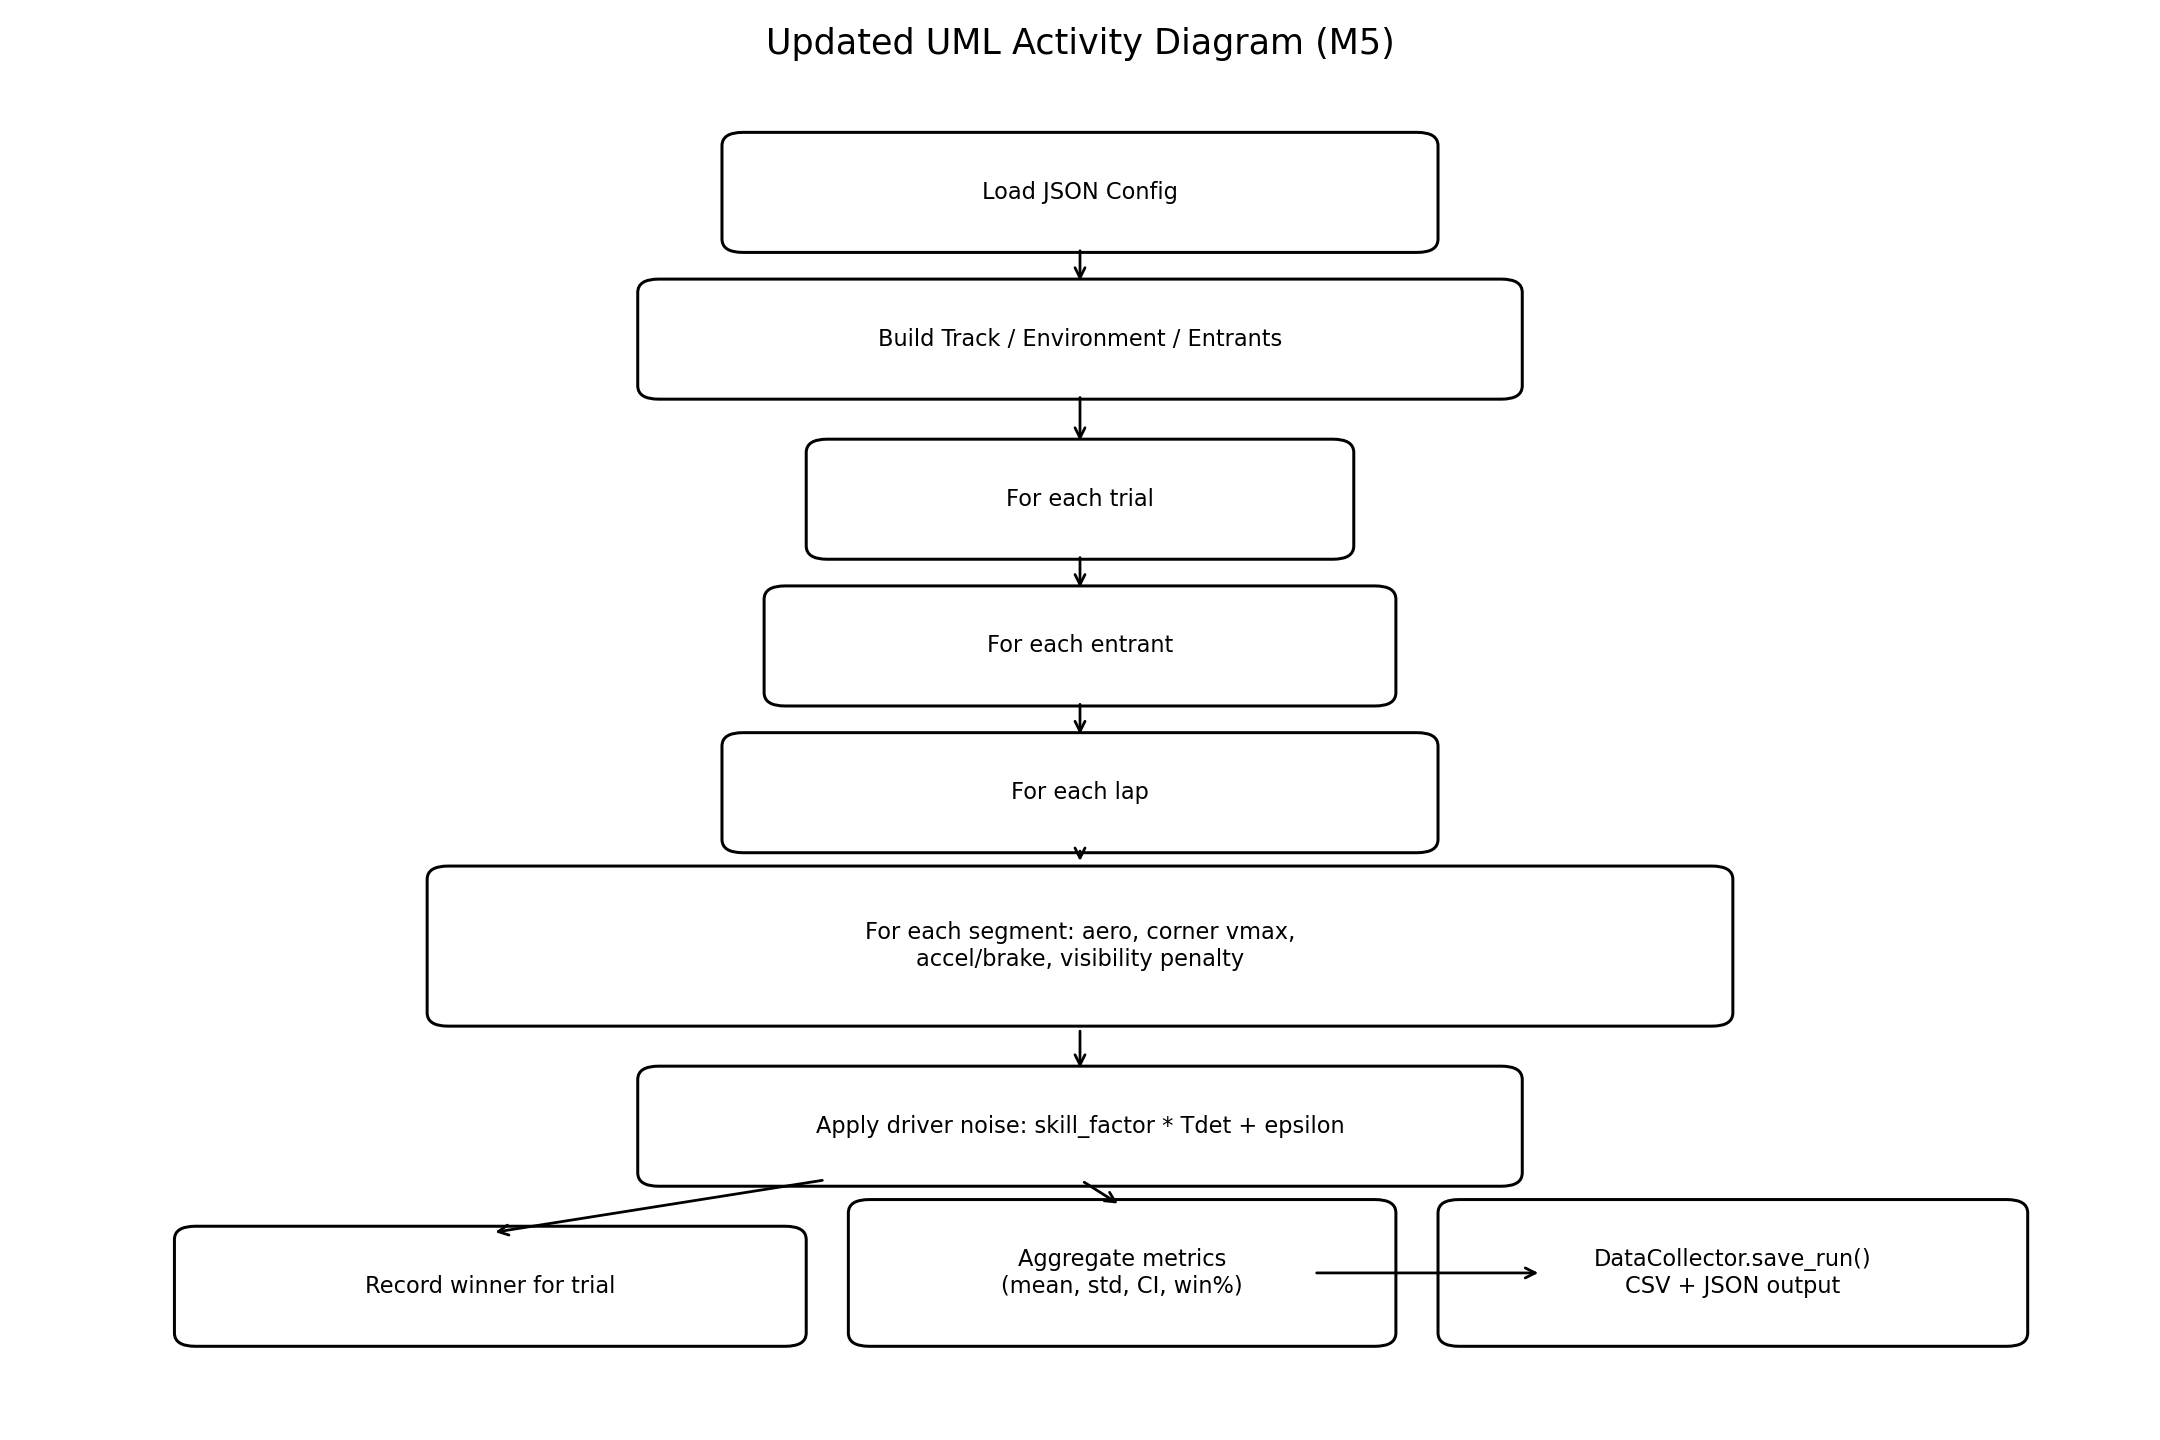
\includegraphics[width=\textwidth]{figures/uml_activity_diagram.png}
    \caption{Updated UML activity diagram showing trial/lap/segment execution flow.}
\end{figure}

\subsection{Key Design Decisions}
\begin{itemize}
    \item Smoothstep blending replaced linear wetness interpolation to reduce binary tire dominance.
    \item N-entrant generalization replaced earlier fixed two-driver assumptions.
    \item Fixed-per-race environment sampling improves experiment control and reproducibility.
    \item DataCollector pipeline was separated from simulation logic for clean outputs and analysis reuse.
\end{itemize}

\section{Implementation}
Implementation is in Python 3.10+ with dataclass-centered models in \texttt{src/}. The simulator core is in \texttt{src/simulation.py}; execution entrypoint is \texttt{main.py}; milestone analysis is in \texttt{m4\_analysis.py}.
Visualization and statistical figures were generated using Matplotlib \cite{matplotlib}.

\subsection{Core Algorithms}
\begin{itemize}
    \item Aerodynamic drag/downforce via quadratic speed model.
    \item Corner speed limit using effective friction and downforce-adjusted normal load.
    \item Traction-limited straight acceleration (\texttt{\_traction\_limited\_accel}).
    \item Grip-aware braking under wetness (\texttt{\_wet\_brake\_decel}).
    \item Visibility penalty applied per segment under low visibility.
    \item Driver stochasticity as Gaussian noise with experience-dependent variance.
\end{itemize}

\subsection{Data Structures and Outputs}
The system uses typed dataclasses for segment, lap, race, and trial results, then exports:
\begin{itemize}
    \item run configuration snapshots,
    \item summary JSON statistics,
    \item lap-level time-series CSV,
    \item segment-level event CSV,
    \item master run index JSON.
\end{itemize}

\subsection{Representative Console Output}
Figures~\ref{fig:example-dry-run} and~\ref{fig:example-wet-run} show representative console output from the baseline dry and wet scenarios used in the final demonstration. These screenshots make the end-to-end execution concrete by showing the printed scenario header, entrant lineup, per-entrant aggregate statistics, best expected performer, execution time, and saved output directory.

\begin{figure}[H]
    \centering
    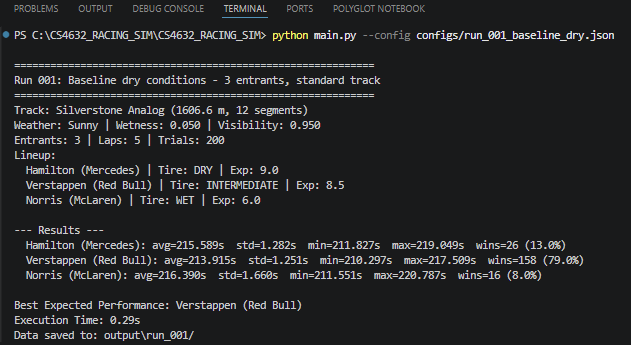
\includegraphics[width=\textwidth]{figures/example_run1.png}
    \caption{Example console output for the baseline dry scenario (Run 001).}
    \label{fig:example-dry-run}
\end{figure}

\begin{figure}[H]
    \centering
    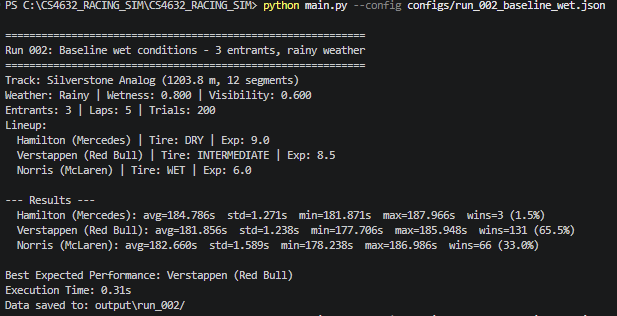
\includegraphics[width=\textwidth]{figures/example_run2.png}
    \caption{Example console output for the baseline wet scenario (Run 002).}
    \label{fig:example-wet-run}
\end{figure}

\section{Experimental Setup}
Experiments are defined by JSON files in \texttt{configs/}. Twelve preset scenarios vary weather, field size, lap count, track complexity, and tire strategy. Baseline conditions use 5 laps and 200 trials with controlled seed values.

Sensitivity analysis varied one factor at a time:
\begin{enumerate}
    \item Wetness,
    \item Visibility,
    \item Number of laps,
    \item Number of Monte Carlo trials,
    \item Track segment-pair count.
\end{enumerate}

Analysis artifacts are generated under \texttt{output/m4\_analysis/} and figures are included in this report.

\section{Results and Analysis}
Representative baseline runs are shown before the sweep figures to ground the later trends in concrete simulator output. In the dry baseline, Verstappen has the best expected total time and dominant win percentage, while the wet baseline shifts all average times and redistributes win rates due to the harsher environment. These screenshots also demonstrate that the simulator reports the exact output directory used for downstream JSON/CSV inspection.

\begin{figure}[H]
    \centering
    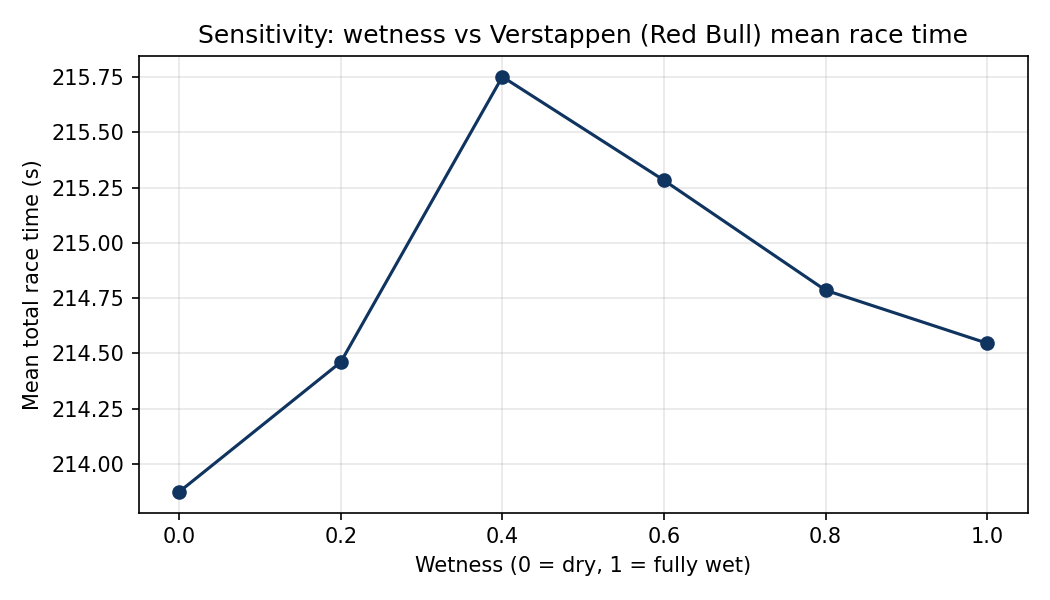
\includegraphics[width=0.86\textwidth]{figures/fig_wetness_vs_time.png}
    \caption{Sensitivity of mean race time to wetness.}
\end{figure}

\begin{figure}[H]
    \centering
    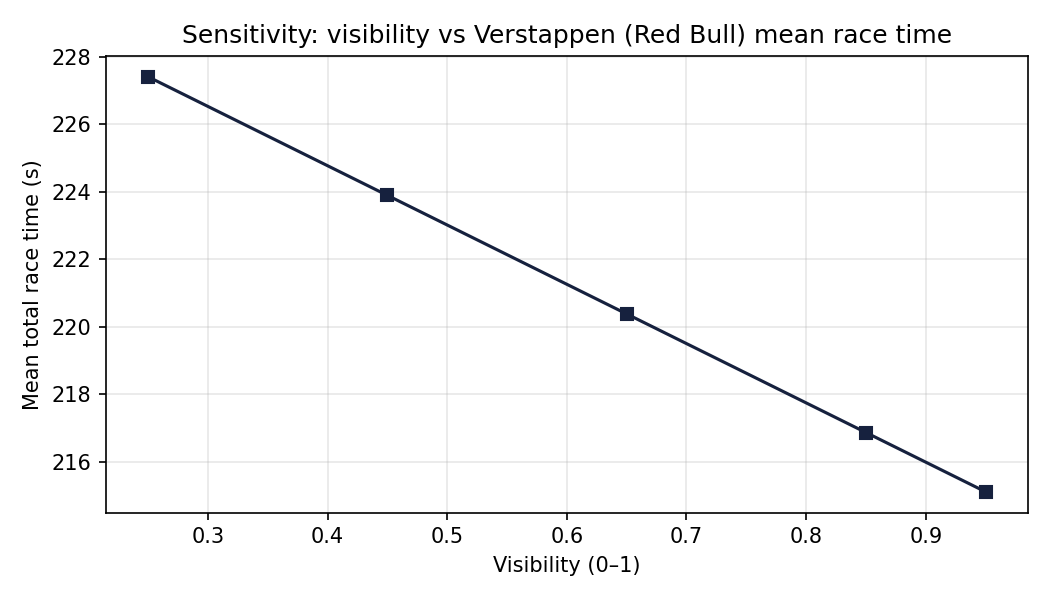
\includegraphics[width=0.86\textwidth]{figures/fig_visibility_vs_time.png}
    \caption{Sensitivity of mean race time to visibility.}
\end{figure}

\begin{figure}[H]
    \centering
    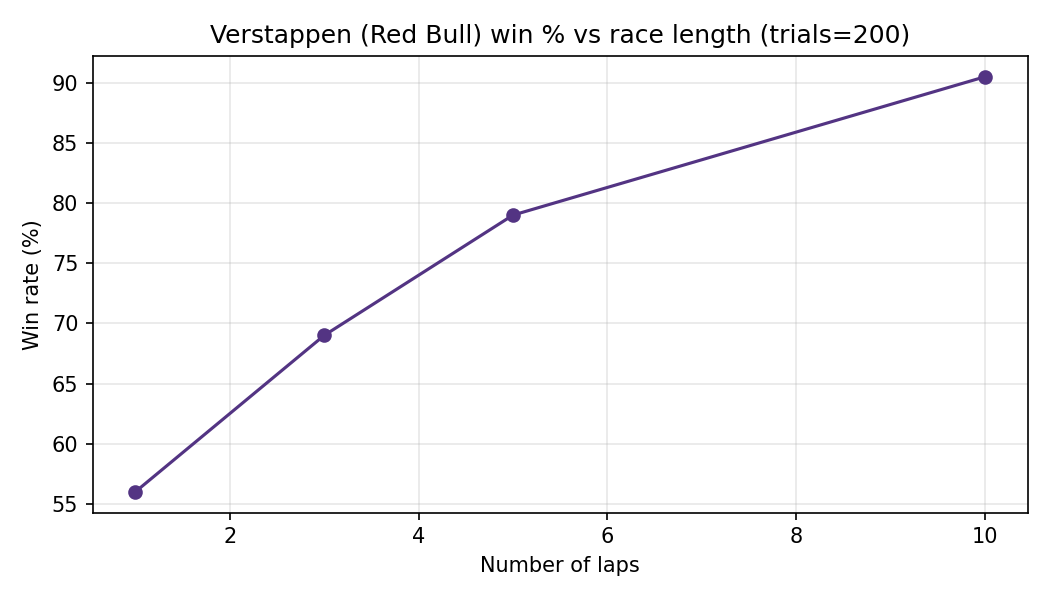
\includegraphics[width=0.86\textwidth]{figures/fig_laps_vs_winpct.png}
    \caption{Win percentage versus race length.}
\end{figure}

\begin{figure}[H]
    \centering
    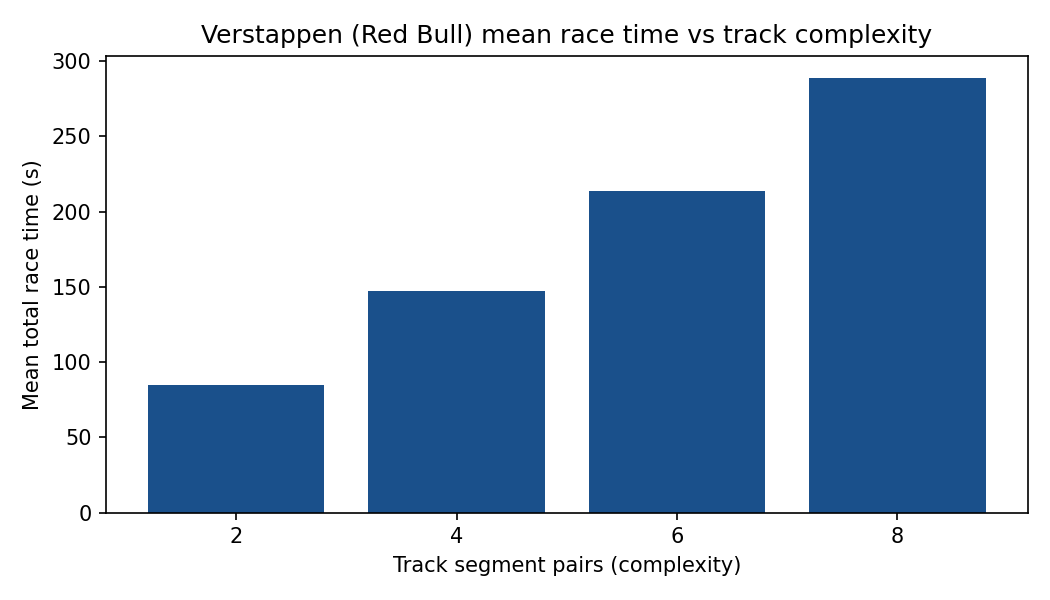
\includegraphics[width=0.86\textwidth]{figures/fig_track_pairs_vs_time.png}
    \caption{Race-time response to track complexity.}
\end{figure}

Key trends:
\begin{itemize}
    \item Wetness shows the strongest nonlinear sensitivity in expected race times.
    \item Visibility introduces moderate penalties but smaller effects than wetness.
    \item Longer race distance stabilizes win-rate signals relative to sprint scenarios.
    \item Track complexity increases aggregate time as expected via additional corner constraints.
\end{itemize}

\begin{table}[H]
    \centering
    \caption{Scenario comparison subset used in milestone analysis (runs 001, 002, 007, 012).}
    \begin{tabular}{ll}
        \toprule
        Run & Scenario focus \\
        \midrule
        001 & Baseline dry \\
        002 & Baseline wet \\
        007 & Sprint race \\
        012 & Foggy mixed strategy \\
        \bottomrule
    \end{tabular}
\end{table}

\section{Validation and Verification}
Validation used three checks:
\begin{itemize}
    \item Parameter-sweep trend sanity (monotonic or expected directional responses),
    \item Trial-count convergence behavior using confidence interval band width,
    \item Qualitative order-of-magnitude comparison against realistic motorsport spread.
\end{itemize}

\begin{figure}[H]
    \centering
    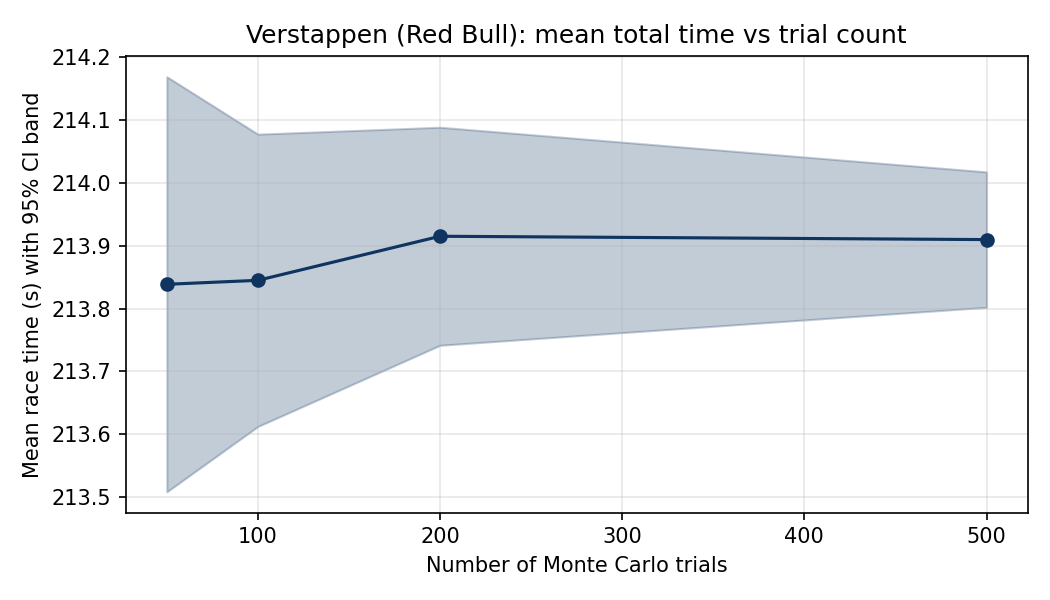
\includegraphics[width=0.86\textwidth]{figures/fig_trials_vs_ci.png}
    \caption{Monte Carlo trial-count effect on confidence interval stability.}
\end{figure}

Limitations are acknowledged: no pit strategy, no tire degradation progression across laps, no mechanical failures, and no full transient vehicle state integration.

\section{Discussion}
The final simulator supports all central project objectives from M1 through M4 and provides a defensible narrative from conceptual design to validated analysis. The most important corrective change during development was rebalancing wetness/tire sensitivity through smoothstep blending and traction/braking model updates. This resolved early over-dominance behavior and produced probabilistic rather than deterministic tire outcomes.

Research questions were addressed as follows:
\begin{itemize}
    \item Environmental inputs (especially wetness) materially change expected race outcomes.
    \item A reduced-order segment model can still yield meaningful and explainable trends.
    \item Stochastic driver variance affects ranking stability and confidence interpretation.
\end{itemize}

\subsection{Integration of Previous Milestones}
This final report integrates and refines all prior milestone work into a single cohesive project narrative. From Milestone 1, it preserves and updates the theoretical foundation, research framing, and UML-based architectural planning. From Milestone 2, it incorporates the key implementation challenges identified during early development, especially model balancing and sensitivity behavior under wet conditions. From Milestone 3, it carries forward the completed simulation system, including generalized N-entrant support, JSON-driven configuration workflows, and structured data export for reproducibility. From Milestone 4, it incorporates the full analysis and validation layer, including one-factor-at-a-time sensitivity studies, scenario comparisons, confidence-interval-driven statistical interpretation, and visualization outputs. Together, these integrated components demonstrate the project’s progression from conceptual design to validated simulation and reproducible analysis.

\section{Conclusion and Future Work}
This project delivered a complete stochastic motorsport simulation pipeline with reusable configuration, robust output collection, and reproducible analysis. Final contributions include N-entrant support, improved wetness/tire balancing, and a structured M4 analytics framework.

Future work should prioritize:
\begin{itemize}
    \item tire degradation over race distance,
    \item pit stop and fuel strategy modeling,
    \item richer powertrain representation (torque/gear effects),
    \item calibration against literature-based or empirical motorsport datasets.
\end{itemize}

\printbibliography[heading=bibintoc,title={References}]

\appendix
\section{Appendix A: Sample Configuration}
\begin{verbatim}
{
  "run_id": "001",
  "description": "Baseline dry conditions",
  "num_laps": 5,
  "num_trials": 200
}
\end{verbatim}

\section{Appendix B: Sample Timeseries Rows}
\begin{verbatim}
trial,lap,entrant,lap_time,cumulative_time,weather,wetness
1,1,Hamilton (Mercedes),25.10234,25.10234,Sunny,0.05
1,2,Hamilton (Mercedes),24.99127,50.09361,Sunny,0.05
1,3,Hamilton (Mercedes),25.18764,75.28125,Sunny,0.05
\end{verbatim}

\section{Appendix C: Smoothstep Friction Blend}
\begin{verbatim}
t = wetness * wetness * (3.0 - 2.0 * wetness)
base_mu = (1.0 - t) * mu_dry + t * mu_wet
\end{verbatim}

\end{document}
